%!TEX root = ../../main.tex

\chapter{Quality of Nanodiamonds}	\label{ch::crystal_quality}
\chaptermark{Quality}

		Carbon exists in a variety of crystalline and disordered structures, exhibiting three hybridizations, sp$^3$, sp$^2$, sp$^1$, see  \Fref{fig::c_bonds}. In its sp$^3$ configuration, characteristic of diamond, each of the four carbon valence electrons are assigned to a tetrahedrally directed sp$^3$ orbital resulting in strong $\sigma$ bonds with adjacent atoms.
		In the three-fold coordinated sp$^2$ configuration of graphite, $\sigma$ bonds form a bonding plane as three of the four valence electrons participate in trigonally directed sp$^2$ orbitals. The remaining fourth electron of the sp$^2$ is found in a p$_z$(p$\pi$) orbital normal to the boding plane. Here $\pi$ orbital form weaker $\pi$ bonds between one or more neighboring atoms.
		The final configuration is denoted sp$^1$ where two out of four valence electrons enter $\sigma$ orbitals. Here $\sigma$ bonds are formed directed along the x-axis. The remaining two electrons participate in p$\pi$ orbitals in the y and z directions.
		Strong directional $\sigma$ bonds give rise to the extreme physical properties of carbon in its diamond form. Graphite is characterized by strong intra-layer $\sigma$ bonding and weak van der Waals bonding across different layers \cite{Robertson2002}.

		\begin{figure}[!htb]
			\centering
			\testbox{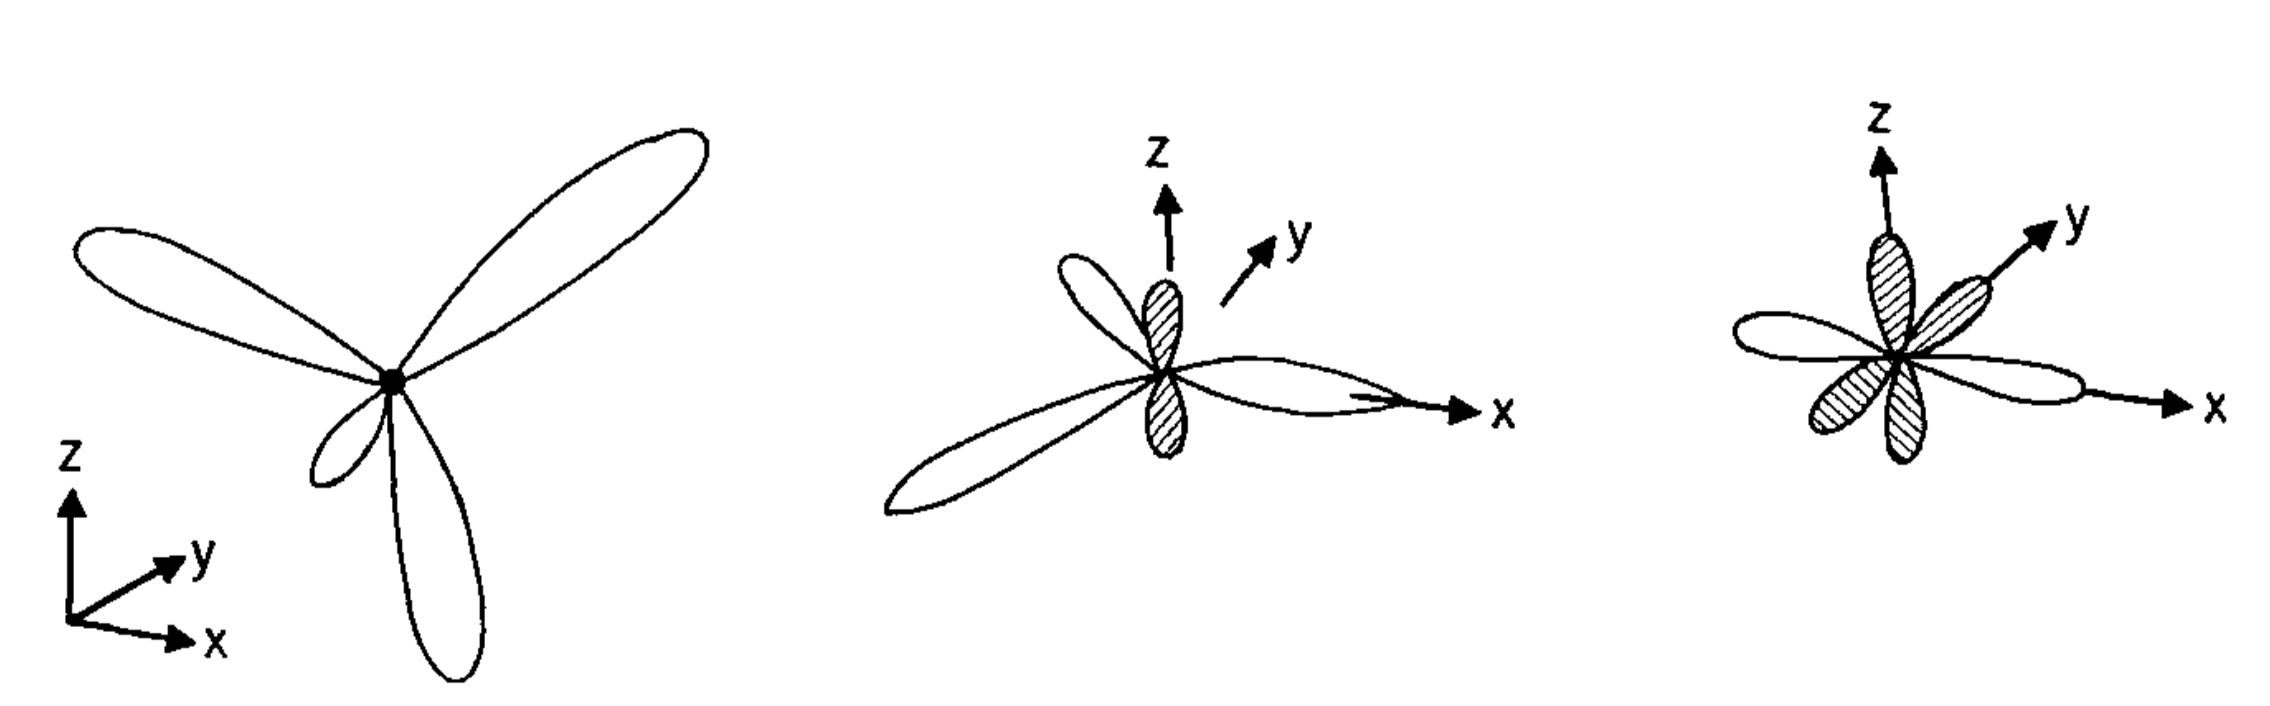
\includegraphics[trim = 0 0 0 0,  clip= true, width = 0.7\textwidth]{./pics/c_bonds_axis.png}}
			\caption[Carbon hybridizations]{The sp$^3$, sp$^2$, sp$^1$ hybridized bonding of carbon \cite{Robertson1986}.}
			\label{fig::c_bonds}
		\end{figure}


		In this thesis we perform measurements of \sivs hosted in \nds produced by various means \Fref{ch::fabrication_nanodiamonds}.
		In this context we use the term quality as a measure of how close diamond crystals are to their pristine form.
		The presence of lattice imperfections such as additional vacancies, lattice strain, impurities or the inclusion of graphite or amorphous carbon is known to adversely affect crystal quality \cite{Zaitsev2001,Prawer2004,Orwa2000}.
		\\
		Surface contamination like graphite and amorphous sp$^2$ hybridized carbon atoms manifest themselves as additional peaks in the Raman spectrum.
		Strain in the diamond lattice broadens the first order Raman peak and causes it to shift to higher or smaller wavenumbers.
		Similarly, high concentrations of lattice defects cause additional peaks, a broadening of the first order Raman peak and a shift towards smaller wavenumbers.
		\\
		To improve crystal quality and to reduce the mentioned distracting effects the following methods are deployed here: Annealing in a vacuum, oxidation in air as well as surface treatments involving plasmas.
		\\
		To study the effectiveness of these treatments and to gauge the quality of our \nd samples we rely on Raman spectroscopy and TEM imaging. The former is used to detect strain, quantify defect concentration and the presence of carbon in non-diamond phases, while the latter enables imaging of individual \nds revealing details in crystallinity such as crystal boundaries.

		\section{Quality-improving Post-Processing Treatments}

			\subsection{Annealing and Oxidation}\label{subsec::ann_ox}

				In this thesis we perform measurements with \nds produced both by direct \CVD growth and by wet-milling a \CVD diamond film.
				In a \cvd reactor, either an amorphous carbon deposit, or a crystalline diamond film may be produced depending on the ratio of the fluxes of carbon and atomic hydrogen onto a substrate \cite{Ford1995,Olson1993}.
				Hence, both the milled and directly grown \nds may be contaminated with amorphous carbon.
				The degree of contamination can be kept to a minimum by tuning the parameters of the growth process.
				\\
				\sivs were formed both via \textit{in-situ} implantation during \CVD growth and via \si implantation.
				\textit{In-situ} implantation disrupts the integrity of the diamond lattice and potentially leads to lattice damage.
				During \si implantation the diamond lattice gets damaged by the penetrating ions.
				sp$^2$ bonds, carbon interstitials and vacancies disrupt the metastable equilibrium of the diamond phase.
				Hence, there is a tendency for damaged diamond to ``tip over" to the thermodynamically stable form of carbon, i.e.\ graphite.
				\\
				At temperatures above about \SI{500}{\celsius}, vacancies in the diamond lattice become mobile and diffuse towards the surface\cite{Dresselhaus1992} disrupting the pristine diamond surface, causing surface contamination.
				Literature suggests, that annealing at \SI{900}{\celsius} for \SI{1}{\hour} is sufficient to remove most of the damage following implantations.
				To reduce the damage in the diamond lattice even further, we anneal the implanted diamonds at \SIrange{900}{1200}{\celsius} for \SIrange{3}{6}{h} in vacuum (\SI{e-6}{Pa}).
				\\
				The surface of the \nds is contaminated with graphite and amorphous sp$^2$ hybridized carbon. In particular, for milled diamonds additional contaminations are commonly introduced by the milling process due to mechanical abrasions. To remove these, we apply oxidation in an oven under ambient air at a temperature of \SI{450}{\celsius} for \SIrange{3}{6}{h}.

			\subsection{Surface Treatment With Gas And Plasma}\label{subsec::plasma}

				% Cardiff
				If contaminations are present on the surface of \nds they can absorb a fraction of the \fl emitted from within the diamond. Thus they reduce the quantum yield of \sivs. We want to explore the possibility of reducing the detrimental effects of surface contaminations via various surface treatments with different gases.
				\\
				In particular, we treated our \nds with hydrogen (\ch{H2}), oxygen (\ch{O2}), ozone (\ch{O3}) both at room temperature and at  \SI{500}{\celsius}. Alternatively, we apply a \ch{H2} plasma\footnote{performed by \williams}.
				\\
				Unfortunately, the only samples that yielded spectra with measurable \ZPLs were the ones treated with \ch{H2}. However, we did not observe any luminescence enhancement.
				\\
				For all other treatments, we found that \nds either did not show any luminescence or immediately bleached upon excitation. Bleaching occurs even when using a continuous wave \SI{660}{nm} laser at low excitation powers of \SI{200}{\micro\watt}. While we cannot say for sure why this the case, we suspect that the treatments favor \siv ionization. Since this approach did not seem fruitful, we did not pursue it further.
				\\
				% C-Schalen
				% One sample showed shells around the \nd after oxidization in air.
				% We attribute this effect to a contamination in the oven.
				% When we illuminated these \nds in the SEM for several moments, the shell went away.
				% We therefore deducted that the shell is organic material.
				% To get rid of the shells on the whole sample, we treated it with oxygen-argon plasma for \SI{3}{min}\footnote{Treatment performed by \schmauch}.
				% After the first treatment, the shells were smaller, but not gone.
				% So we put them into the oxygen-argon plasma again for \SI{3}{min}, however, the shells were bigger than before any treatment.
				% We tried another approach to get rid of the shells with ozone treatment for \SI{4}{\hour} at \SI{360}{\celsius}.
				% Before ozone treatment there the diamond Raman line and other Raman lines visible.
				% After surface treatment, more lines appeared and all of these other lines got more intense.
				% There are probably organic contaminations on the sample in which functional groups got introduced by the ozone treatment.
				% We did not further investigate this sample and defined it as broken.

		\section{Raman Measurements} \label{sec::raman}

			Raman spectroscopy of various samples gives insight into crystal quality and surface contamination of \nds.
			Raman scattering is the inelastic scattering of a photon $\hbar\omega_i$ on a molecule or crystal lattice in the initial state $\ket{i}$ with energy $E_i$.
			The molecule of crystal transitions into a higher energy state $E_f$ and the scattered photon with frequency $\omega_s$ looses the energy $\Delta E = E_f - E_i = \hbar(\omega_i-\omega_s)$.
			Therefore, energy is exchanged between the photon and the excited matter, changing the rotational or oscillation energy of the involved molecule or the oscillation energy, i.e.\ phonons of the crystal lattice.
			The Raman shift is typically referenced in wavenumbers and given by
			% 
			\begin{equation}
				\Delta \omega = \left( \frac{1}{\lambda_{ex}}-\frac{1}{\lambda_R}\right).
			\end{equation}

			As every solid exhibits characteristic phonon modes tied to the properties of its lattice structure, Raman spectroscopy can be used to characterize diamond.
			Raman measurements of \nds give insight into the issues of surface contamination, lattice strain and defect concentration:
			Surface contamination like graphite and amorphous sp$^2$ hybridized carbon atoms cause additional peaks in the Raman spectrum.
			A high defect concentration may lead to additional peaks, a broadening of the first order Raman peak and a shift to smaller wavenumbers.
			Strain in the diamond broadens the first order Raman peak and causes a shift to higher wavenumbers \cite{Zaitsev2001,Prawer2004,Orwa2000}.
			\\
			For Raman measurements the setup described in \Fref{sec::confocal} is used.
			As excitation light source, a \SI{532}{nm} continuous wave diode laser operating in single mode is used (Integrated Optics\textregistered Matchbox Laser 0532L-41B).
			It provides single frequency mode laser light, a prerequisite for Raman investigations.
			The beamsplitter is a dichroic mirror (DRLP645), the laser light is additionally blocked out with a \SI{532}{\nm} notch filter in the detection path in front of the single mode fiber replacing the usual long pass filter.
			With these adaptations, the combination of the confocal unit and the spectrometer serves as a Raman spectrometer.
			As the diamond Raman line is very narrow, the \SI[per-mode=symbol]{600}{\lines\per\mm} grating does not offer sufficient resolution and is only used for a coarse approach. Detailed measurements are realized using \SI[per-mode=symbol]{1200}{\lines\per\mm} and \SI[per-mode=symbol]{1800}{\lines\per\mm} gratings.
			\\

			% Versuchsdurchfuehrung
			Since the size of single \nds is on the order of tens of nanometers, low signal intensities can become an issue when taking Raman measurements.
			To overcome this problem we pursue two different approaches:
			\begin{enumerate}[label=\alph*),ref=\alph*)]
				\item \Nd Clusters: \label{item::raman_gband} Collective measurements are carried out at several areas on the sample \insituS. Since this sample is densely covered with \nds, collective measurements of clusters of \nds (\Fref{subfig::raman_no}) achieve higher signal intensities.
				\item Large \Nds: \label{item::raman_implanted} Raman measurements are carried out on the implanted sample \implantedTao. For this sample, diamond particles are large enough to yield sufficient intensities on single \nds.
			\end{enumerate}

			\begin{figure}[!htp]
				\begin{subfigure}{0.5\linewidth}
					\centering
					\testbox{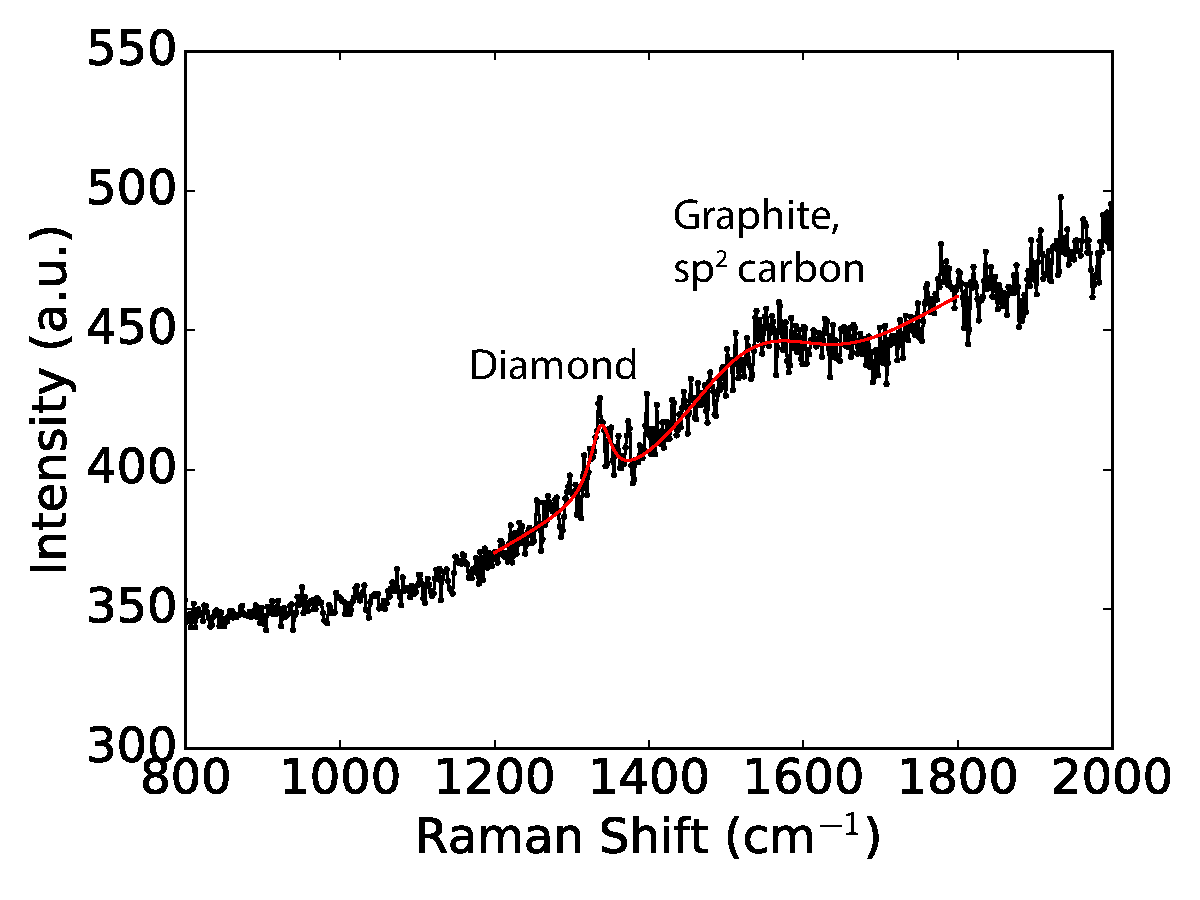
\includegraphics[trim = 0 0 0 0 , clip = true, width = \pairplotwide]{./pics/Ir25_spectrum_scan_xy-05x6y8_4000uW_t60_wavenumber_fit.pdf}}
					\caption{}\label{subfig::raman_no}
				\end{subfigure}
				\hfill
				\begin{subfigure}{0.5\linewidth}
					\centering
					\testbox{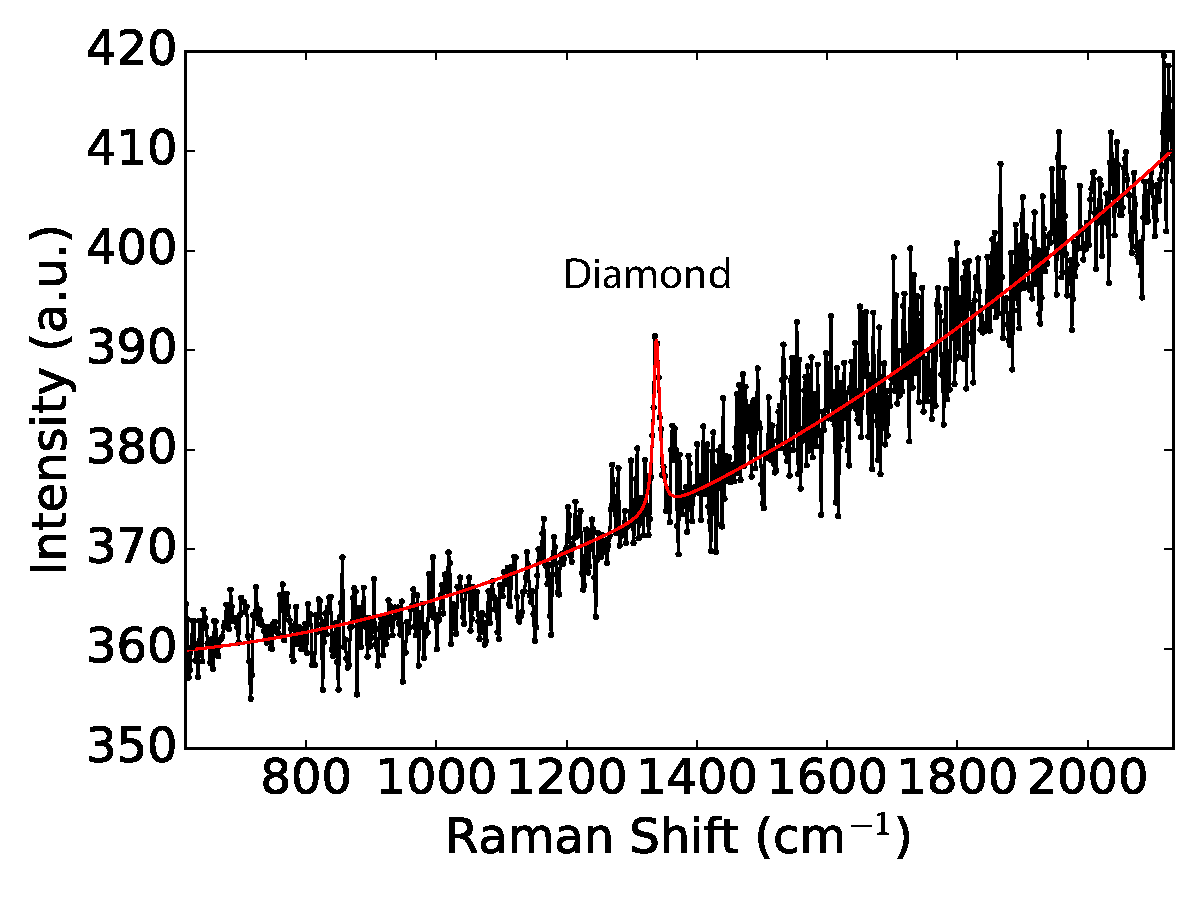
\includegraphics[trim = 0 0 0 0,  clip = true, width = \pairplotwide]{./pics/Ir_22_spe_scan_xy-02x7y7_550-600nm_t240_wavenumber_fit.pdf}}
					\caption{}\label{subfig::raman_ox}
				\end{subfigure}
				\caption[Raman spectrum of a single \nd]{Raman measurements, black: data, red: fit. (a) Raman measurement before oxidation, sample \insituS. The diamond Raman peak is situated at \SI{1338}{\per\centi\meter}. The broad feature around \SI{1580}{\per\centi\meter} corresponds to the graphite G-band. (b) Raman measurement after oxidation, sample \insituSo. The G-band has vanished, indicating removal of graphite and amorphous sp$^2$ hybridized carbon.}
				\label{fig::raman}
			\end{figure}

			\subsection{Surface Contamination}\label{subsec::raman_surface_contamination}

				We test the impact of oxidation treatment as described in \Fref{subsec::ann_ox} on surface contamination.
				\Fref{subfig::raman_no} shows a measured Raman spectrum of a sample without oxidation treatment (\insituSn).
				To verify reproducibility, the measurement is performed on three different spots of the sample.
				The narrow peak in \Fref{subfig::raman_no} corresponds to the first order diamond Raman peak and will be further analyzed in \Fref{subsec::raman_strain}.
				The spectrum also shows a broad peak with a Raman shift of about \SI[separate-uncertainty]{1582+-5}{\per\centi\meter}.
				This shift corresponds to the G-band due to amorphous sp$^2$ hybridized carbon atoms and graphite.
				The exact G-band position and \lw is sensitive to parameters such as the clustering of the sp$^2$ phase, bond-length and bond-angle disorder, presence of sp$^2$ rings or chains, and the sp$^2$/sp$^3$ ratio \cite{ferrari2004raman}.
				The \nd Raman spectra are considerably modified after \ox in air at \SI{450}{\degreeCelsius}.
				To verify this, we perform Raman measurements on three different spots of a sample produced in the same process as the above mentioned, which is additionally oxidized (\insituSo).
				While the G-band peak is present in every measurement performed on a non-oxidized sample, it is not present in any of the oxidized samples (\Fref{subfig::raman_ox}), indicating successful removal of sp$^2$ hybridized carbon and surface graphite.

			\subsection{Defect Concentration}\label{subsec::raman_defect_concentration}
				
				Several effects impact the first order diamond Raman line:
				\begin{enumerate*}
					\item defects in the diamond lattice,
					\item hydrostatic pressure,
					\item uniaxial or more complicated stress configurations.
				\end{enumerate*}
				In the measurement on \nd clusters the width of the diamond Raman peak of sample \insituS varies between \SIlist{15; 30}{\per\centi\meter} without \ox treatment, but is only \SIrange{9}{11}{\per\centi\meter} after the \ox process.
				A possible reason for this change of the width is improved crystal quality \cite{Prawer2004}.
				In the measurement on large \nds we measured a Raman line at \SI[separate-uncertainty]{1308+-5}{\per\centi\meter} (denoted line R1) which exhibits a broad \lw of \SI[separate-uncertainty]{25+-5}{\per\centi\meter}.
				One plausible explanation for both the position and the \lw of the Raman line are defects in the diamond lattice \cite{Prawer2004}.

			\subsection{Lattice Strain}\label{subsec::raman_strain}

				We investigated how strain in the diamond lattice manifests itself in both measurements on \nd clusters and on large \nds.
				In the Raman measurement on \nd clusters, the position of the diamond Raman peak is the same for oxidized (\insituSo) and non-oxidized (\insituSn) samples, indicating that oxidation does not affect strain in the diamond.
				However, the Raman shift of both non-oxidized and oxidized samples amounts to \SI[separate-uncertainty]{1338+-5}{\per\centi\meter}, as compared to the literature value of \SI{1332.5}{\per\centi\meter} of pristine diamond \cite{Zaitsev2001} (given uncertainties are governed by spectrometer resolution).
				This shift indicates the presence of strain in the diamond particles.
				\\
				Performing Raman measurements on large \nds we find diamond Raman lines at \SI[separate-uncertainty]{1308+-5}{\per\centi\meter} (line R1), at \SI[separate-uncertainty]{1345+-5}{\per\centi\meter} (line R2) and at \SI[separate-uncertainty]{1348+-5}{\per\centi\meter} (line R3), indicating a broad distribution of strain among the individual diamond particles (uncertainties governed by spectrometer resolution).
				Only line R1 can be explained with a high defect concentration in the diamond lattice due to its shift to smaller \wl.
				\todo{determine differences to paper and resolve. Active text is from paper, commented from thesis.}
% 
				% However, a more consistent model which explains all occurring shifts is the presence of strain in the diamond nano particles.
				% From the \lws in the measurement on large \nds, the strain in the diamond is calculated using the equation for hydrostatic pressure \cite{Prawer2004} given by
				% % 
				% \begin{equation}
				% 	\omega(P)=\omega_0+a_1P+a_2P^2,
				% \end{equation}

				% where $\omega_0=\SI{1332.5}{\per\centi\meter}$, $a_1=\SI{2.83}{\per\centi\meter\per\giga\pascal}$ and $a_2=\SI{-3.65e-3}{\per\centi\meter\per\giga\pascal}$.
				% The calculation yields a pressure in the investigated diamonds of \SI{-8.56}{\giga\pascal} tensile stress and \SIlist{4.26;5.50}{\giga\pascal} compressive stress.
				% Pressure uncertainties due to the Raman line measurements are smaller than one Pascal and are therefore neglected.
				% Under hydrostatic pressure, the triply degenerate first order Raman peak remains degenerate, while under uniaxial and more complex stress configurations (biaxial stress, shear stress etc.) mode splitting occurs \cite{Prawer2004}.
				% As mentioned above, we observe broad \lws up to \SI[separate-uncertainty]{25+-5}{\per\centi\meter}.
				% The broad \lws of the Raman lines may be attributed to uniaxial strain, as mode splitting manifests itself in a broadening of the peak due to limited spectrometer resolution.
				% Therefore, we conclude that both hydrostatic and uniaxial strain is present in the \nds.
% 
				However, a more consistent model which explains all occurring shifts is the presence of strain/stress in the diamond nanoparticles. The Raman shift $\Delta \nu$ in the presence of compressive and tensile stress is given by \cite{Widmann2016,Liscia2013a}: 
% 
				\begin{equation}
					\Delta \nu = \frac{p}{0.34},
				\end{equation}

				where the Raman shift $\Delta\nu$ is given in \SI{}{\per\centi\meter} and the stress $p$ in \SI{}{\giga\pascal}. 

				The calculation yields a pressure range from \SI[separate-uncertainty]{-8.33+-1.7}{\giga\pascal} tensile stress to \SI[separate-uncertainty]{5.27+-1.7}{\giga\pascal} compressive stress. Whereas under hydrostatic pressure the triply degenerate first order Raman peak remains degenerate, under uniaxial and more complex stress configurations (biaxial stress, shear stress etc.) mode splitting occurs \cite{Prawer2004}. As mentioned above, we observe broad \lws up to \SI[separate-uncertainty]{25+-5}{\per\centi\meter}.
				The broad \lws of the Raman lines may be attributed to uniaxial strain, as mode splitting manifests itself in a broadening of the peak due to limited spectrometer resolution.

		\section{Transmission Electron Microscopy}{\label{sec::tem}}

			Transmission electron microscopy (\TEM, also sometimes conventional transmission electron microscopy or CTEM) is a microscopy technique in which a beam of electrons is transmitted through a specimen to form an image. The specimen is most often an ultra-thin section less than \SI{100}{\nm} thick or a suspension on a grid. An image is formed through the interaction of the electrons with the sample as the beam is transmitted through the specimen.
			Since electrons have higher de Broglie wavelengths than photons, a higher resolution is obtainable, allowing the surface of \nds to be resolved. Thus, the crystallinity of single \nds can be studied directly.


			\subsection{Crystallinity and Grain Boundaries}\label{subsec::tem_crystal}

				For \TEM investigations \nd samples must obey certain size requirements.
				In particular, they must be large enough for the carbon grid inside the microscope acting as a stage for specimen to hold them.
				Furthermore, their diameter must not exceed a certain value, since the \TEM electron beam must be able to permeate the material for imaging.
				Samples of type \insituH mostly comprised of \nds fulfilling these requirements, was investigated by \schmauch.
				\\
				In \Fref{subfig::tem_crystal} a \TEM image of a single \nd is shown. A complex crystal formation deviating from single crystal diamond structure is visible. A higher resolution detail is given in \Fref{subfig::tem_boundary}. The image clearly shows different crystal orientations, asserting that the \nd particle is not a single crystal diamond. Within the nanodiamond, several sharp lines are visible. These lines are edges of crystal boundaries and grain boundaries, introducing strain in the diamond lattice. We remark at this point that some studies suggest the possibility that \sivs are created with a higher probability at grain boundaries and morphological defects of the crystal \cite{bray2016localization, zapol2001tight}.
				\\
				We have repeated this visual assessment of crystal quality for a range of different \nds with identical results. This supports the conclusion that all of our \nds are polycrystalline specimen.

				\begin{figure}[!htb]
					\begin{subfigure}{ 0.49\linewidth}
						\centering
						\testbox{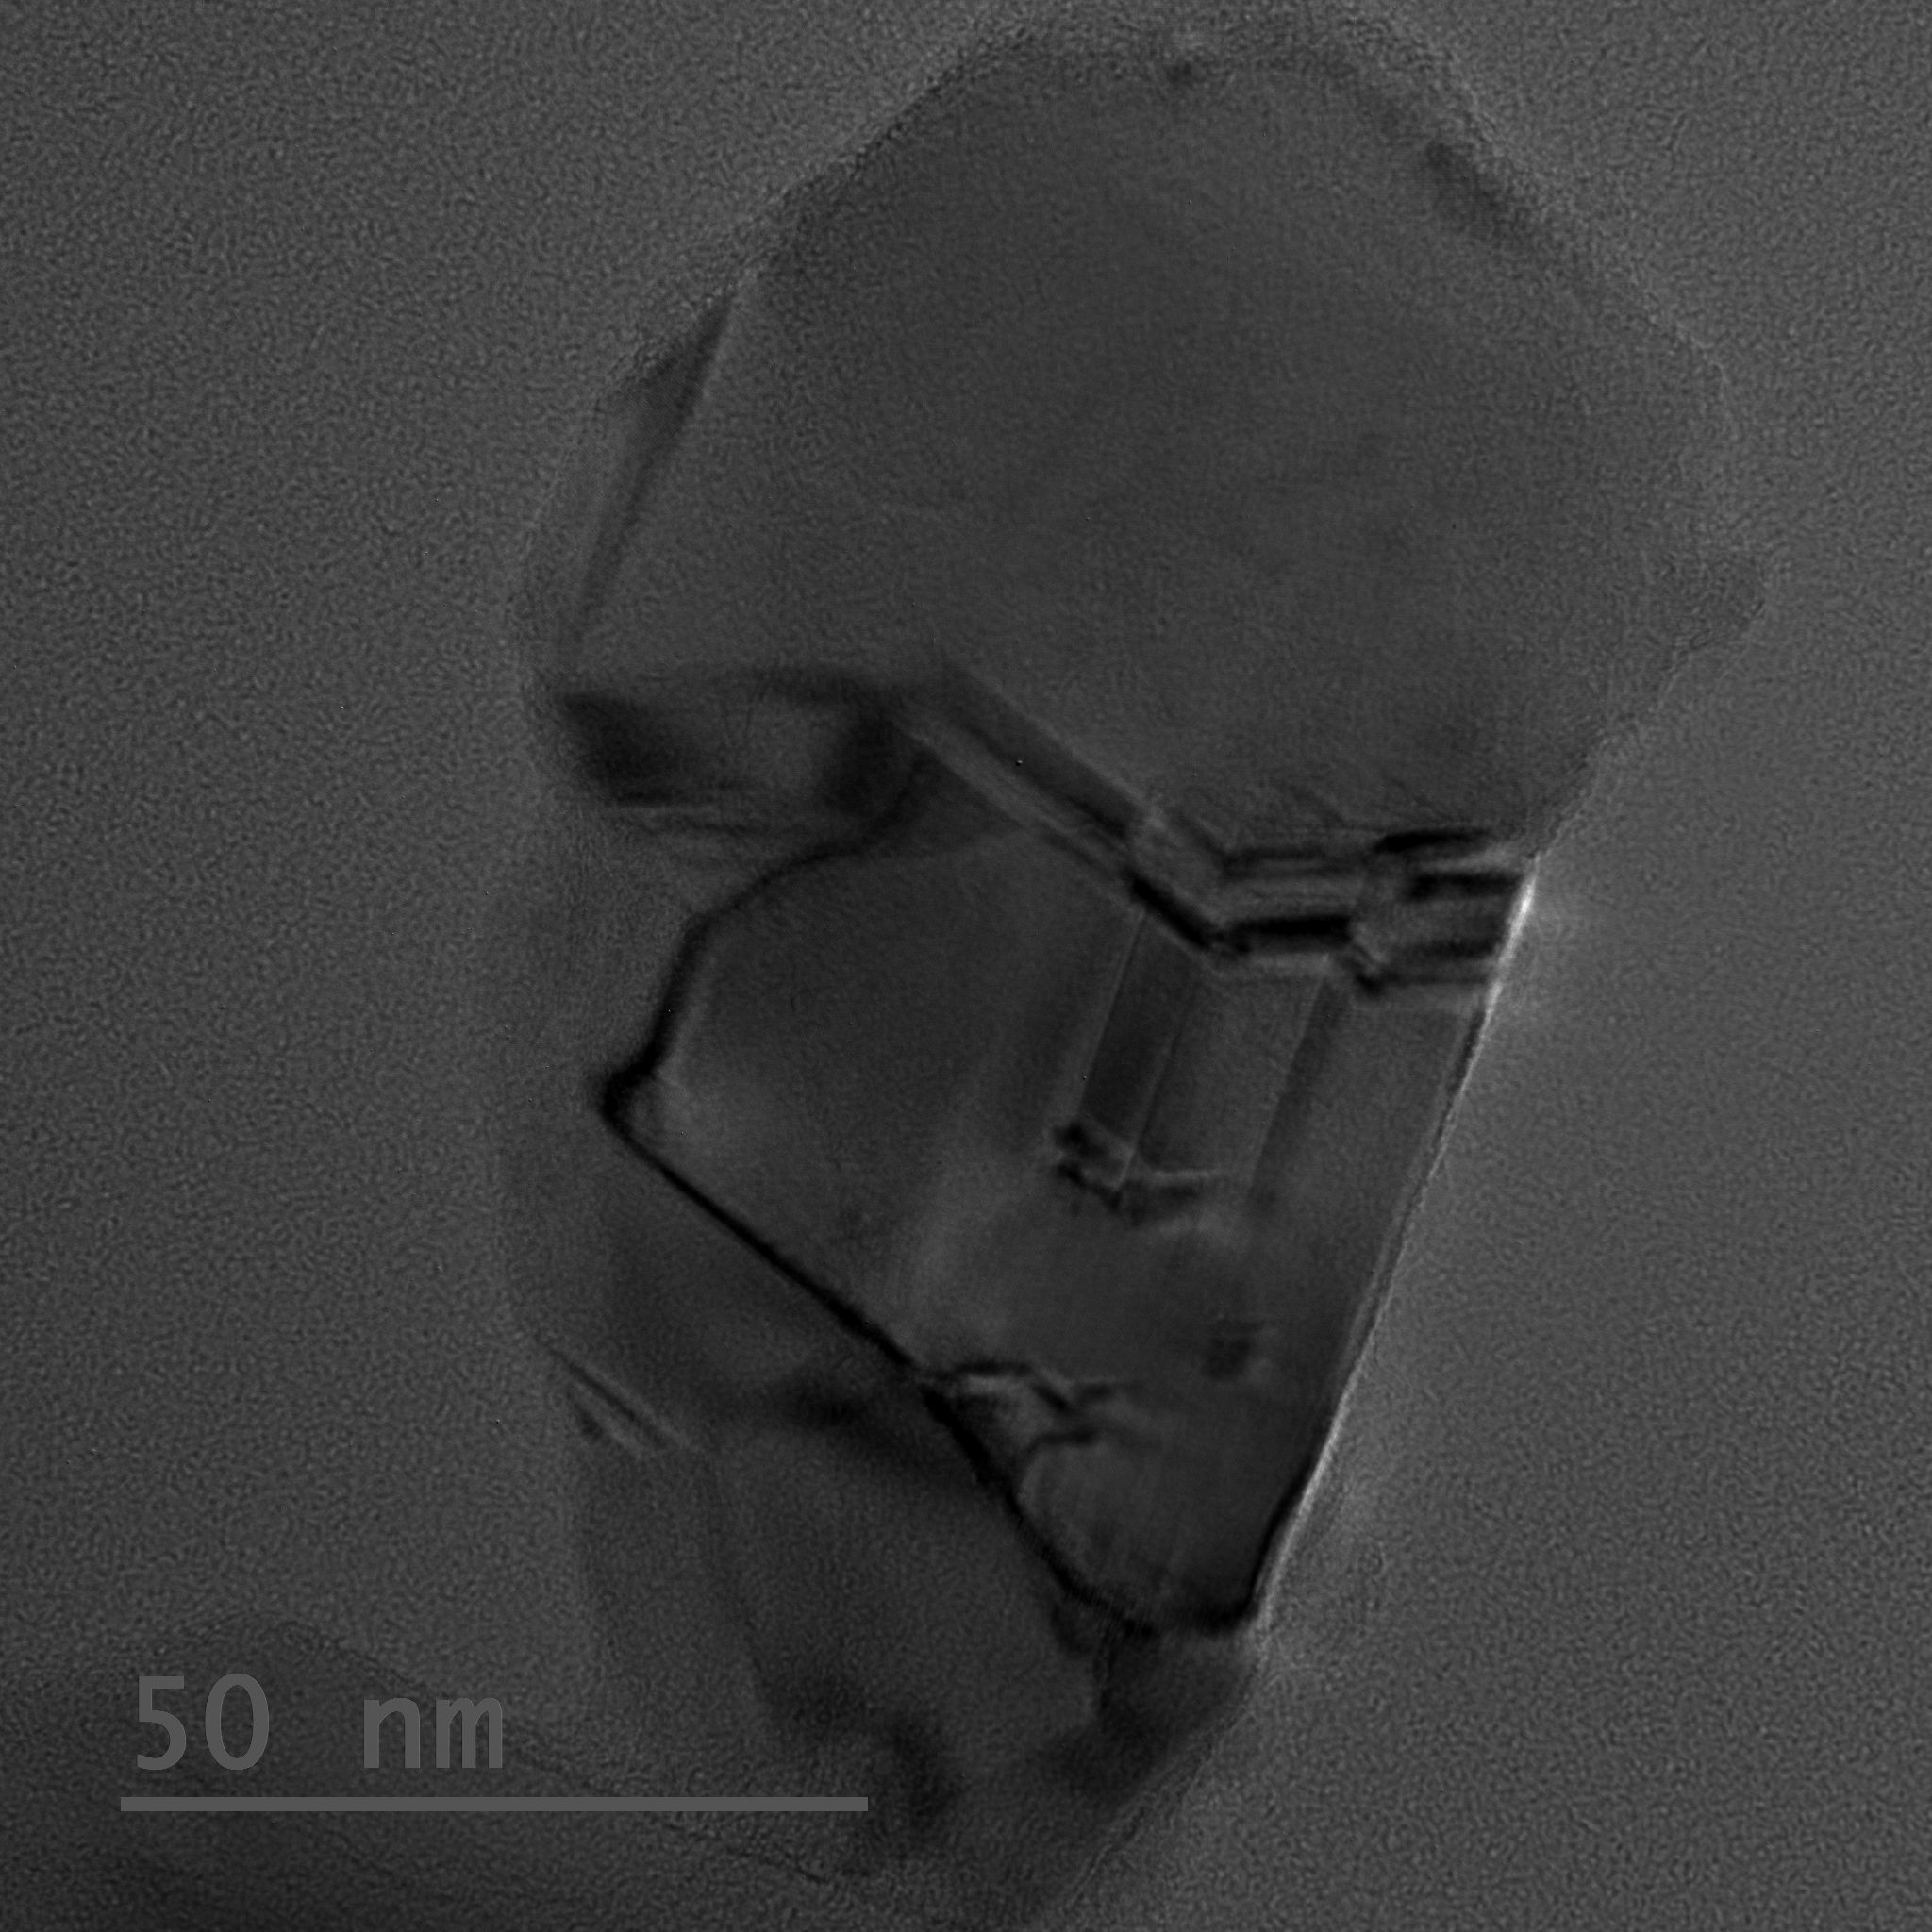
\includegraphics[trim = 0 0 0 0,  clip= true, width = \pairplotwide]{./pics/AM060-II-k4-2.png}}
						\caption{}
						\label{subfig::tem_crystal}
					\end{subfigure}
					\hfill
					\begin{subfigure}{ 0.49\linewidth}
						\centering
						\begin{tikzpicture}
							\begin{scope}[spy using outlines={rectangle,red,magnification=2.5,size=2.5cm}]
							\node{\testbox{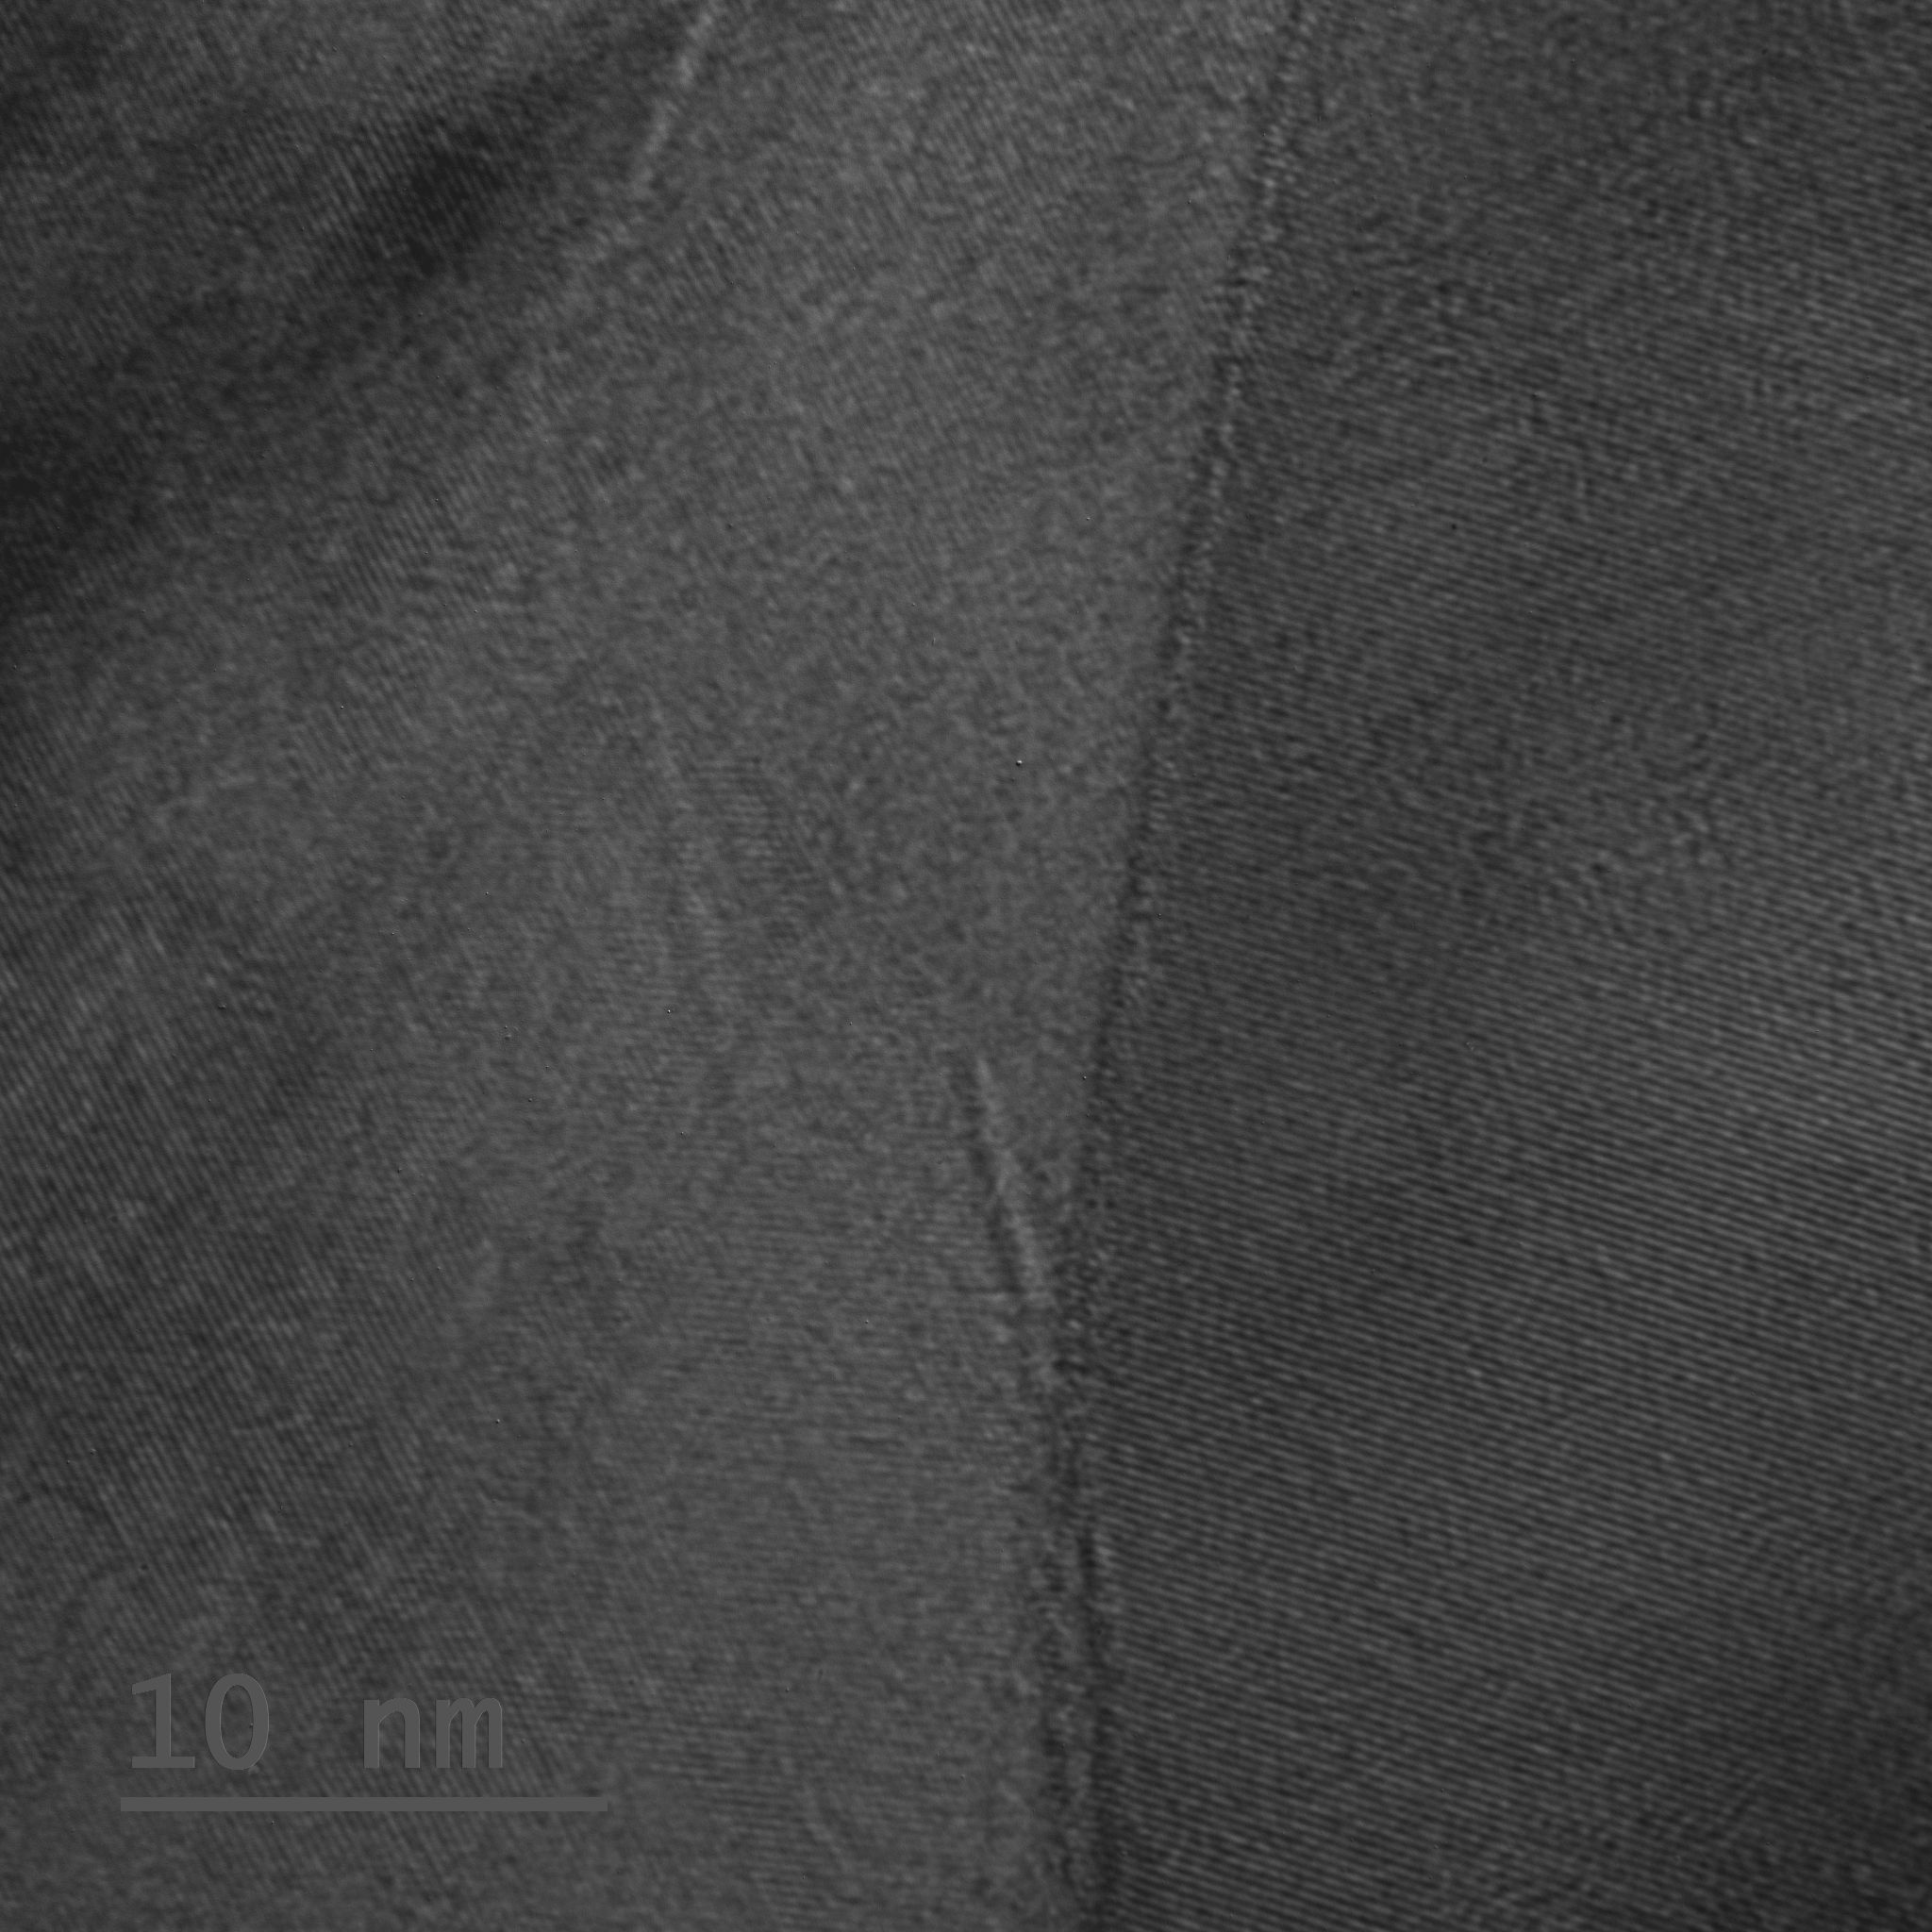
\includegraphics[trim = 0 0 0 0,  clip= true, width = \pairplotwide]{./pics/AM060-II-k1-3.png}}};
							\spy on (1.0,2) in node (a) [left] at (2.7,-1.5);
							\end{scope}
						\end{tikzpicture}
						\caption{}
						\label{subfig::tem_boundary}
					\end{subfigure}
					\caption[\TEM imaging of a single \nd]{Transmission electron microscopy (TEM) pictures of sample \insituH. (a) Image of a single \nd particle revealing a complex crystal structure. (b) Close-up image a diamond particle. The vertical line is a crystal boundary, to the left and right the parallel layers of one crystalline region can be seen. For better visibility, the inset shows a magnification of the area indicated by a red box. The different orientations of the crystal lattice layers is visible.}
					\label{fig::tem}
				\end{figure}
